\section{I colori}

Come stabilito in fase di pianificazione, l'applicazione verterà su un colore rosso-arancio, in quanto solitamente associato alla nota di Do. 

Si è, quindi, generata una \emph{palette} di colori partendo da un colore arancio scuro, simile al colore dei cachi. Si sono scelti quattro colori seguendo la ``regola'' della tetrade cromatica, selezionando dei colori con una distanza di trenta gradi circa (sulla ruota cromatica) dal colore principale.

Si veda la tabella \ref{tab:palette} per avere dei riferimenti visivi sui colori scelti. Per ogni colore, sono presentate quattro tinte diverse (escludendo il colore ``puro'', mostrato in posizione centrale) e sono riportati i vari codici in esadecimale. Inoltre, è possibile osservare la resa sia di un testo bianco che di uno nero sulle varie tinte.

\renewcommand{\arraystretch}{1.5}
\begin{table}[H]
	\centering
	\caption[Palette dei colori]{\emph{Palette} dei colori su cui è basato il \emph{design} di \ProjectTitle{}}
	\label{tab:palette}
	\begin{tabular}{lccccc}
		\hline
		{\footnotesize Colore primario:}       & \cellcolor[HTML]{FF9E6B}{\begin{tabular}[c]{@{}c@{}}{\color[HTML]{FFFFFF} \texttt{\#FF9E6B}}\\ \texttt{\#FF9E6B}\end{tabular}} & \cellcolor[HTML]{FF8C4F}{\begin{tabular}[c]{@{}c@{}}{\color[HTML]{FFFFFF} \texttt{\#FF8C4F}}\\ \texttt{\#FF8C4F}\end{tabular}} & \cellcolor[HTML]{E55100}{\begin{tabular}[c]{@{}c@{}}{\color[HTML]{FFFFFF} \texttt{\#E55100}}\\ \texttt{\#E55100}\end{tabular}} & \cellcolor[HTML]{802D00}{\begin{tabular}[c]{@{}c@{}}{\color[HTML]{FFFFFF} \texttt{\#802D00}}\\ \texttt{\#802D00}\end{tabular}} & \cellcolor[HTML]{571E00}{\begin{tabular}[c]{@{}c@{}}{\color[HTML]{FFFFFF} \texttt{\#571E00}}\\ \texttt{\#571E00}\end{tabular}} \\ \hline
		{\footnotesize Colore secondario (1):} & \cellcolor[HTML]{FFC56B}{\begin{tabular}[c]{@{}c@{}}{\color[HTML]{FFFFFF} \texttt{\#FFC56B}}\\ \texttt{\#FFC56B}\end{tabular}} & \cellcolor[HTML]{FFB94F}{\begin{tabular}[c]{@{}c@{}}{\color[HTML]{FFFFFF} \texttt{\#FFB94F}}\\ \texttt{\#FFB94F}\end{tabular}} & \cellcolor[HTML]{E58B00}{\begin{tabular}[c]{@{}c@{}}{\color[HTML]{FFFFFF} \texttt{\#E58B00}}\\ \texttt{\#E58B00}\end{tabular}} & \cellcolor[HTML]{804D00}{\begin{tabular}[c]{@{}c@{}}{\color[HTML]{FFFFFF} \texttt{\#804D00}}\\ \texttt{\#804D00}\end{tabular}} & \cellcolor[HTML]{573500}{\begin{tabular}[c]{@{}c@{}}{\color[HTML]{FFFFFF} \texttt{\#573500}}\\ \texttt{\#573500}\end{tabular}} \\ \hline
		{\footnotesize Colore complementare:}    & \cellcolor[HTML]{6FABEF}{\begin{tabular}[c]{@{}c@{}}{\color[HTML]{FFFFFF} \texttt{\#6FABEF}}\\ \texttt{\#6FABEF}\end{tabular}} & \cellcolor[HTML]{4D8DD5}{\begin{tabular}[c]{@{}c@{}}{\color[HTML]{FFFFFF} \texttt{\#4D8DD5}}\\ \texttt{\#4D8DD5}\end{tabular}} & \cellcolor[HTML]{0C4D95}{\begin{tabular}[c]{@{}c@{}}{\color[HTML]{FFFFFF} \texttt{\#0C4D95}}\\ \texttt{\#0C4D95}\end{tabular}} & \cellcolor[HTML]{012853}{\begin{tabular}[c]{@{}c@{}}{\color[HTML]{FFFFFF} \texttt{\#012853}}\\ \texttt{\#012853}\end{tabular}} & \cellcolor[HTML]{001B39}{\begin{tabular}[c]{@{}c@{}}{\color[HTML]{FFFFFF} \texttt{\#001B39}}\\ \texttt{\#001B39}\end{tabular}} \\ \hline
		{\footnotesize Colore secondario (2):} & \cellcolor[HTML]{64EFC5}{\begin{tabular}[c]{@{}c@{}}{\color[HTML]{FFFFFF} \texttt{\#64EFC5}}\\ \texttt{\#64EFC5}\end{tabular}} & \cellcolor[HTML]{42D6A9}{\begin{tabular}[c]{@{}c@{}}{\color[HTML]{FFFFFF} \texttt{\#42D6A9}}\\ \texttt{\#42D6A9}\end{tabular}} & \cellcolor[HTML]{00976A}{\begin{tabular}[c]{@{}c@{}}{\color[HTML]{FFFFFF} \texttt{\#00976A}}\\ \texttt{\#00976A}\end{tabular}} & \cellcolor[HTML]{00543B}{\begin{tabular}[c]{@{}c@{}}{\color[HTML]{FFFFFF} \texttt{\#00543B}}\\ \texttt{\#00543B}\end{tabular}} & \cellcolor[HTML]{003928}{\begin{tabular}[c]{@{}c@{}}{\color[HTML]{FFFFFF} \texttt{\#003928}}\\ \texttt{\#003928}\end{tabular}} \\ \hline
	\end{tabular}%
\end{table}
\renewcommand{\arraystretch}{2}

Ai precedenti colori, vanno poi aggiunti i colori bianco (\colorbox[HTML]{FFFFFF}{\texttt{\#FFFFFF}}), nero (\colorbox{black}{\color{white}\texttt{\#000000}}) e grigio all'80\% (\colorbox[HTML]{333333}{\color{white}\texttt{\#333333}}), utilizzati per contrastare i colori più accesi e per il testo dell'applicazione.

\section{Le gabbie logiche}

Come fase preliminare al design dell'applicazione vera e propria, il team ha condotto una fase di \emph{brainstorming} che aveva come obiettivo la definizione delle varie sezioni (grafiche) dell'applicazione. Frutto di tale processo sono le seguenti gabbie logiche, che definiscono la struttura basilare che è stata scelta per l'applicazione.

\begin{figure}[H]
	\centering
	\begin{subfigure}[t]{0.5\textwidth}
		\centering
		
\includegraphics[width=\textwidth]{gabbie_logiche/Landing_Page}
		\caption{La \emph{landing page}}
	\end{subfigure}%
	~ 
	\begin{subfigure}[t]{0.5\textwidth}
		\centering
		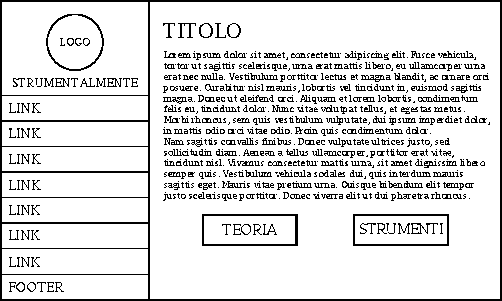
\includegraphics[width=\textwidth]{gabbie_logiche/Home}
		\caption{La \emph{home page}}
	\end{subfigure}
	\begin{subfigure}[t]{0.5\textwidth}
		\centering
		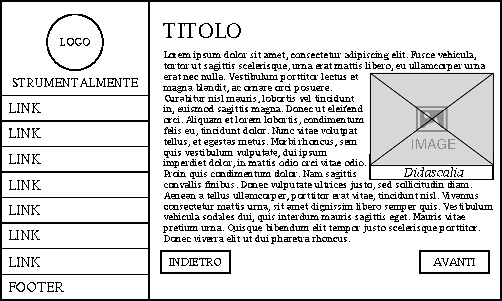
\includegraphics[width=\textwidth]{gabbie_logiche/Contenuto_Generico}
		\caption{La struttura delle pagine dei contenuti}
	\end{subfigure}%
	~ 
	\begin{subfigure}[t]{0.5\textwidth}
		\centering
		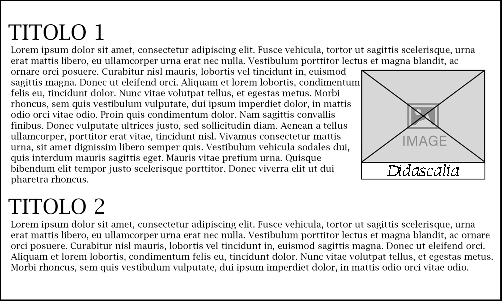
\includegraphics[width=\textwidth]{gabbie_logiche/Aiuto}
		\caption{La pagina \emph{(pop-up)} di aiuto, di bibliografia e altro}
	\end{subfigure}
	\begin{subfigure}[t]{0.5\textwidth}
		\centering
		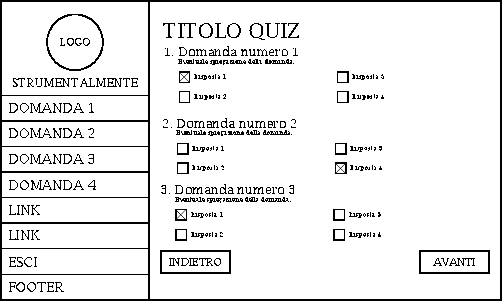
\includegraphics[width=\textwidth]{gabbie_logiche/Pagina_Quiz}
		\caption{Una pagina del \emph{quiz}}
	\end{subfigure}%
	~ 
	\begin{subfigure}[t]{0.5\textwidth}
		\centering
		
\includegraphics[width=\textwidth]{gabbie_logiche/Risultati_Quiz}
		\caption{La pagina \emph{(pop-up)} dei risultati del \emph{quiz}}
	\end{subfigure}
	\begin{subfigure}[t]{0.5\textwidth}
		\centering
		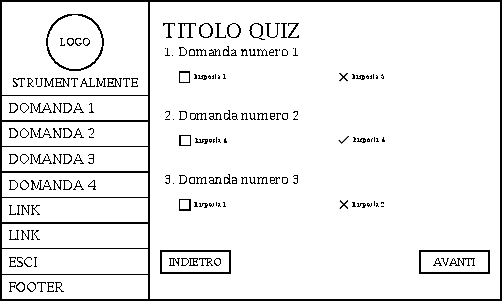
\includegraphics[width=\textwidth]{gabbie_logiche/Controlla_Quiz}
		\caption{Una pagina di controllo del \emph{quiz}}
	\end{subfigure}
	\label{fig:gabbie-logiche}
	\caption{Le gabbie logiche di \ProjectTitle{}}
\end{figure}

\section{Le icone}

Come prestabilito, l'applicazione deve avere un \emph{look} moderno e accattivante. A tale scopo si è scelto di seguire alcune linee guida dettate dal \emph{Material Design} di \emph{Google}. A tal fine, si è scelto di utilizzare delle icone semplici simili, per l'appunto, a quelle che \emph{Google} consiglia per creare applicazioni in \emph{Material Design}. 

Con uno sguardo teso alla fase di realizzazione del sistema, si sceglie di utilizzare le icone fornite dal \emph{font} \emph{Font Awesome}\footnote{\url{https://fontawesome.com/}}, in quanto sono disponibili diverse icone, gratuitamente disponibili, che rispettano gli standard imposti per la creazione di \ProjectTitle{}.